% !TEX root = /Users/orhankoc/Documents/optima/internal-docs/latex/revenue-management

\documentclass[conference,letterpaper]{IEEEtran}
\usepackage[letterpaper, left=1in, right=1in, bottom=1in,
top=0.75in]{geometry}\usepackage[utf8]{inputenc}
\usepackage{multirow}
\usepackage{ntheorem}
\usepackage{graphicx}
\usepackage{amsmath}
\usepackage{ upgreek }
\renewcommand{\arraystretch}{2}

\title{Algorithmic Capital Allocation for Decentralized Applications}
\author{\IEEEauthorblockN{Orhan Koc}
    \IEEEauthorblockA{ hankoc@onchainfactory.com} }

\date{December 2021}

\begin{document}
    \maketitle
    \begin{abstract}
        With the advent of blockchain technology, ownership of purchasing power can be
        proved without a trusted central entity. This fundamental advancement has made it
        possible to build semi algorithmic companies, paving the way for a new paradigm.
        As is the case with multi-division companies, determining the optimal funding
        strategy of a decentralized application is a crucial component for its growth.
        This paper attempts to automate the department funding process of cryptocurrency
        applications by proposing a configurable, KPI based optimization algorithm to
        compare alternatives and adjust funding.
    \end{abstract}

    \section{Introduction}
        Early age of cryptocurrency projects used to be composed of a financial service
        which incurs a fee to the user. As the advantages of blockchain based services
        became more apparent, the design of such applications became more complex, with
        multiple revenue and expense streams added such as the token, application
        treasury, node operators et cetera. The newly added corporate structures to simple
        cryptocurrency applications had a lot of technical debt, in that applications
        failed to implement common corporate finance strategies in their organization. The
        seperation of these sub-divisions in cryptocurrency applications warrant a clear
        identification of a comparison framework to evaluate the returns of revenue
        allocation alternatives. 
        
        It's important to note this paper isn't about capital budgeting, which describes
        how capital is spent within a sub-division; for example what percentage of the
        treasury should be allocated for operational expenses, or which venture to acquire
        in the presence of excess cash. Rather it attempts to automate the decision making
        process of allocating between sub-divisions, distributing available capital to
        ensure the strategic plan is met.

        \subsection{Literature Review}
            Capital allocation within portfolios is an extensively researched field,
            focusing on optimizing a portfolio with respect to risk and capital
            constraints. 

            \subsubsection{CAPM}
            [TODO]

            \subsubsection{Utility Theory}
            [TODO]

            Capital Allocation in decentralized applications is fairly limited due to the
            relatively recent emergence of advancements in blockchain space. Because of
            the experimental nature of decentralized applications, budgeting of these
            financial systems have rather been on the safer side of the spectrum.

            \subsubsection{Revenue compartmentalization} occurs when funds generated by a
            sub-division are used only within that sub-division. An example would be to
            buy and burn tokens using token transfer fees alone.

            \subsubsection{Hardcoding} is a simple technique of budgeting by allocating
            revenue to sub-divisions as predetermined fractions with no updates. Even
            though it is a fairly fool-proof strategy to allocate funds, the lack of
            adaptability to market conditions render this technique suboptimal. This
            approach is parallel to history-based capital allocation where ratio of funds
            allocated are equal to that of previous year.

            \subsubsection{DAO Voting} is a democratic fund allocation process where every
            token counts as one vote. The idea is more stake in the system should equal
            more authority in making decisions. This approach is very similiar to
            Participatory Budgeting which is a paradigm that empowers residents to
            directly decide how a portion of the public budget is spent
            \cite{aziz2021participatory}.


        \subsection{Proposal}
            The fundamentals layed out in portfolio management models and asset pricing
            models \cite{portfolioSelection} have been useful in modeling risk and return
            of assets bearing risk. Even though the risk and return of company
            sub-divisions differ from that of an asset's, there have been successful
            attempts at modeling budgeting algorithms using portfolio management theories
            \cite{cetingoz}. Based on utility theory of assets and aforementioned
            portfolio management models, we propose a standardized, data-driven algorithm
            to decide the captital allocation share for each sub-division of a modern
            cryptocurrency application.
            \begin{center}
                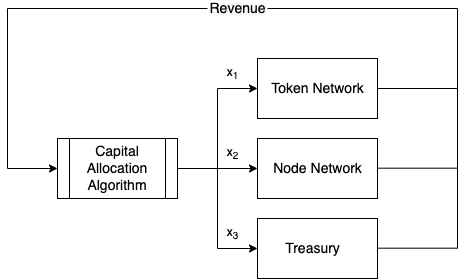
\includegraphics[width=0.45\textwidth]{assets/high_level_capital_allocation.png}
                \textit{Fig. 1 High-Level Revenue Flow}
            \end{center}
            The success of a capital allocation strategy is determined by whether Key
            Performance Indicators (KPIs) as proposed by the executive board are met or
            not. We propose to formulate a capital allocation algorithm in the form of an
            optimization problem for $n$ sub-divisions and maximize the utility of
            expenditures on sub-divisions, utility defined as the percent completion of
            KPI target per dollar spent ($u_n$) with respect to funds allocated ($x_n$). 
            
            In order to provide a general form of the algorithm, the application under
            investigation is composed of 3 sub-divisions: Nodes, Token Holders and
            Treasury.
            
            We will then specify constraints for this optimization problem based on
            budgets imposed on \textbf{Capital} and \textbf{Risk} to specify the solution
            space. In the end, we will have a model with decision variables as funds
            allocated ($x_n$) to subdivision $n$ and implement an iterative process to
            solve for the optimal value of capital allocation that maximizes the expected
            return on KPIs per dollar spent.
        
    \section{Theory}
        \textbf{Expected Utility}
        We can use the Utility function to evaluate quantify how useful an s expenditure is to each

        \textbf{Optimization Model}
        We first acknowledge that we are trying to optimize for the maximum utility given
        limited resources to a set of options that results in unexpected returns. The
        decision of allocation is irrevocable and is conducted periodically with a
        countable step size, where each step depends on the decision made on previous
        steps.

        The most common way to approach a budgeting problem is to use Linear optimization
        with expenditure alternatives as decision variables with a set objective to
        maximize or minimize. The general form for linear optimization model is as follows:

        Minimize or maximize:
        \begin{equation}
            Z = \sum_{i=1}^{n} c_i x_i
        \end{equation}

        Subject to:
        \begin{equation}
            \sum_{i=1}^{n} a_i x_i \le b_i;
        \end{equation}

        Where $Z$ is the objective function subject to minimization or maximization, $c_1,
        c_2, ..., c_n$ are the coefficients of the corresponding decision variables, $x_1,
        x_2, ..., x_n$ are the decision variables we are solving for, $a_1, a_2, ..., a_n$
        are the constraint coefficients and $b_1,b_2, ..., b_n$ are the constraints.

    \section{Model}
        \subsection{Basic setting}
            The challenge of formulating a capital allocation optimizaton problem for a
            decentralized application is to find a single objective function that is
            applicable for different sub-divisions. The simplest example is that the
            performance of a Treasury is measured in terms of Return on Investment, but
            that of a node network is measured in terms of staking percentage.

            The variables($x_i$) are simply the expenditure on a sub-divisions. The
            variable coefficients($c_i$) should represent the weight of the sub-divisions'
            expenditure to the objective. The constraints can be modified to fit the needs
            of specific cases. The constraints, denoted in Equation 2, are the constraints
            that must be satisfied in order for a solution to be considered feasible in
            the linear optimization problem.

        \subsection{Design}
            The main goal of using such an algorithm would be to reach the
            \textit{strategic plan} determined by the executive board. In order for the
            strategic plan to be applicable to the aforementioned optimization model, the
            plan should include performance targets for the Treasury, Node and Token.

            \subsubsection{Variable Coefficients} 
                Essentially, we want to maximize KPI target completion per dollar spent on a
                sub-division. To model this objective, we need a complementary coefficient
                that will convey the relationship between expenditure on sub-division and
                performance increment, $\alpha_i$.
                \begin{center}
                    \begin{tabular}{|p{1.5cm}|p{2cm}|p{1.5cm}|}
                        \hline
                        \textit{-} & \textit{KPI ($P$)}& \textit{ $\Updelta$ KPI} \\
                        \hline
                        Treasury& Growth \%      & $\frac{S_t}{C_{t}}$  \\
                        Token   & Inflation \%   & $\frac{M_t - B_t}{T_{t-1}}$  \\
                        Node    & Stake \%       & $\frac{L_t - U_t}{S_{t-1}}$  \\
                        \hline
                    \end{tabular}
                \end{center}
                \textbf{For treasury}, $R_t$ is the revenue of the protocol added to the
                treasury and equals $x_1$, $E_t$ is the expenses that are deducted from
                treasury  and $C_{t-1}$ is the treasury size at the previous observation
                so that $\Updelta$ $C_t$ is the numerator.
                \newline
                \textbf{For token}, $M_t$ is the amount of newly minted tokens, $B_t$ is
                the amount of newly burned tokens and $T_{t-1}$ is the total amount of
                tokens in circulation at the previous observation so that $\Updelta$ $T_t$
                is the numerator.
                \newline
                \textbf{For node}, $L_t$ is the amount of newly staked tokens, $U_t$ is
                the amount of newly unstaked tokens and $C_{t-1}$ is the total amount of
                staked tokens at the previous observation so that $\Updelta$ $S_t$ is the
                numerator.
                
                Our objective is to maximize the total rate of improvement with respect to
                performance targets.

                \[c_i = \frac{\alpha_i}{P_t - P_i}\] $c_i$ represents expected incremental
                improvement in KPI per dollar in expenditure. $P_t$ $P_c$
                

            \subsubsection{Objective}
                
                \[Z = \frac{\alpha_i}{P_t - P_i} x_i\] 

                It's important to realize KPIs chosen should be directly affected by the
                sub-division expenditure($x_n$). For example the funds spent on token
                inflation, utilized by buying the tokens from the market and burning them,
                have a direct effect on the inflation: the number of tokens put into
                circulation divided by number of tokens removed from circulation. Instead,
                if we are to use token price as a KPI for tracking funds spent on the
                token network the outcome would be noisy, as the price is affected by many
                other parameters.
                \newline

            \subsubsection{Constraints}

            From a capital allocation perspective, probabilistic constraints of the model
            correspond to the limits on how much fund can be spent on each subnetwork.


            The most common seperation of these limits as seen in portfolio optimization
            models are the \textbf{Risk Constraint} and \textbf{Budget Constraint}, which
            can also be applied in this context. \textbf{Risk Constraint} defines the
            maximum 
            \textbf{Budget Constraint}

            \subsection{Solution Method}

    \section{Implementation}
        For the sake of simplicity, we will consider the simplest cryptocurrency
        application with three essential divisons: token network, node network and the
        treasury. 

    \section{Conclusion}


    \subsection{Results}

    \subsection{Evaluation}

    \subsection{Limitations}

    \newpage
    \bibliographystyle{ieeetr}
    \bibliography{citation} 


\end{document}
